\section{Fourierreihen periodischer Funktionen}
	\subsection{Bausteine}
		\textbf{Idee:}\\[3pt]
		$T$-Periodische, mit Limes stückweise stetigen Funktionen, durch Aufsummieren ebenfalls periodischer Basisfunktionen
		(sin, cos) zu approximieren.\\[3pt]

		\textbf{Basisfunktionen:}\\[3pt]
		\begin{minipage}[b]{0.5\textwidth}
			\begin{tabular}{llll}
				Konstante: & $cos(0 \cdot \omega_{f} t) = 1$ & &\\[3pt]
				$1 \times$ Frequenz $f$  & $\cos(1 \cdot \omega_{f} t)$ & ; & $\sin(1 \cdot \omega_{f} t)$\\[3pt]
				$2 \times$ Frequenz $f$: & $\cos(2 \cdot \omega_{f} t)$ & ; & $\sin(2 \cdot \omega_{f} t)$\\[3pt]
				$3 \times$ Frequenz $f$: & $\cos(3 \cdot \omega_{f} t)$ & ; & $\sin(3 \cdot \omega_{f} t)$\\[3pt]
				usw. & & &\\[3pt]
			\end{tabular}
		\end{minipage}
		\begin{minipage}[]{0.5\textwidth}
			\scalebox{0.8}{\begin{tikzpicture}
	%axis
	\begin{scope} [decoration={border, segment length=1cm, amplitude=1mm, angle=90}]
		\draw[postaction={decorate, draw}] (-5, 0) -- (5.1, 0);
		\draw[postaction={decorate, draw}] (0, 0) -- (0, 5.1); 
	\end{scope}
	
	\def\lzero{(-5, 1) cos (-2.5, 1.5) sin (0,2) cos (2.5, 1.5) sin (5, 1)};
	\fill[cyan, opacity=0.2] \lzero;
	\draw[cyan!75!black] \lzero node[right, black] {$\Psi_0(x)$};
	
	\def\lone{(-5, 2.5) cos (-3.33, 2.25) sin (-1.66, 2) cos (0, 2.5) sin (1.66, 3) cos (3.33, 2.75) sin (5, 2.5)}
	\fill[red, opacity=0.2] \lone;
	\draw[red!75!black] \lone node[right, black] {$\Psi_1(x)$};
	
	\def\ltwo{(-5, 4) cos (-3.75, 4.25) sin (-2.5, 4.5) cos (-1.25, 4) sin (0, 3.5) cos (1.25, 4) sin (2.5, 4.5) cos (3.75, 4.25) sin (5, 4)}
	\fill[green, opacity=0.2] \ltwo;
	\draw[green!75!black] \ltwo node[right, black] {$\Psi_2(x)$};
	
	\draw (0, 0) parabola (5, 5);
	\draw (0, 0) parabola (-5, 5);
	
	\draw[latex-latex, red] (-5, -1.5) -- (5, -1.5);
	\node[above, red] at (0, -1.5) {$T = \dfrac{2 \pi}{\omega_f}$ von $f$};
	
	\draw[dashed, red] (-5, -1.5) -- (-5, 5);
	\draw[dashed, red] (5, -1.5) -- (5, 5);
\end{tikzpicture}}
		\end{minipage}\\[3pt]
		\fbox{
			\begin{tabular}{ll}
				Frequenz: & $f = \dfrac{1}{T}$\\[7pt]
				Kreisfrequenz: & $\omega_f = 2 \pi f$\\[3pt]
				Periodendauer: & $T = \dfrac{2 \pi}{\omega_f} = \dfrac{1}{f}$\\[6pt]
				Nullphasenwinkel: & $\varphi$\\[6pt]
			\end{tabular}
		}
	
	\subsection{Berechnung der Fourierkoeffizienten (in $\mathbb{R}$)}
		\textbf{Die Funktion $f(t)$ soll durch folgende Linearkombination dargestellt werden:}\\[3pt]
		\fbox{$FR[f(t)] = \dfrac{a_0}{2} + \sum\limits_{n=1}^{\infty} [a_n \cdot \cos(n \omega_f t) + b_n \sin(n \omega_f t)]$}\\[3pt]
		\begin{minipage}[t]{0.5\textwidth}
			\textbf{Berechnung von $a_0$, $a_n$ und $b_n$\\[1pt] (Fourierkoeffizienten):}\\[3pt]
			\begin{tabular}{|lll|l|}
				\hline
				$\displaystyle a_0$ & $=$ & $\displaystyle \dfrac{2}{T} \cdot \int\limits_{0}^{T} f(t) dt$ & $\displaystyle n = 0$\\[0.2pt]
				\hline
				$\displaystyle b_0$ & $\displaystyle =$ & $\displaystyle 0$ & $\displaystyle n = 0$\\
				\hline
				$\displaystyle a_n$ & $\displaystyle =$ & $\displaystyle \dfrac{2}{T} \cdot \int\limits_{0}^{T} f(t) \cdot \cos(n \omega_f t) dt$ & $\displaystyle n = 0, 1, 2, \cdots$\\
				\hline
				$\displaystyle b_n$ & $\displaystyle =$ & $\displaystyle \dfrac{2}{T} \cdot \int\limits_{0}^{T} f(t) \cdot \cos(n \omega_f t) dt$ & $\displaystyle n = 1, 2, 3, \cdots$\\
				\hline
			\end{tabular}
		\end{minipage}
		\begin{minipage}[t]{0.5\textwidth}
			\textbf{Orthogonalitätsbeziehungen:\\[1pt]}\\[3pt]
			\begin{tabular}{|l|}
				\hline
				$\displaystyle \int\limits_{0}^{T} \cos(m \omega_f t) \cdot \cos(n \omega_f t) dt = \left\lbrace 
					\begin{array}{ll}
						T & \text{für: } m = n = 0\\
						\dfrac{T}{2} & \text{für: } m = n > 0\\
						0 & \text{für: } m \neq n\\
					\end{array} \right.$\\[3pt]
				$\displaystyle \int\limits_{0}^{T} \sin(m \omega_f t) \cdot \sin(n \omega_f t) dt = \left\lbrace 
					\begin{array}{ll}
						\dfrac{T}{2} & \text{für: } m = n > 0\\
						0 & \text{für: } m \neq n\\
					\end{array} \right.$\\[3pt]
				$\displaystyle \int\limits_{0}^{T} \sin(m \omega_f t) \cdot \sin(n \omega_f t) dt = 0$\\[3pt]
				\hline
			\end{tabular}
		\end{minipage}
	
	\subsection{Sätze zur Berechnung der Fourierkoeffizienten}
		\subsubsection{Symmetrie}
			\begin{minipage}[]{0.5\textwidth}
				\begin{tabular}{|c|c|}
					\hline
					\textbf{Gerade Funktion} & \textbf{Ungerade Funktion}\\[3pt]
					\hline
					\scalebox{0.45}{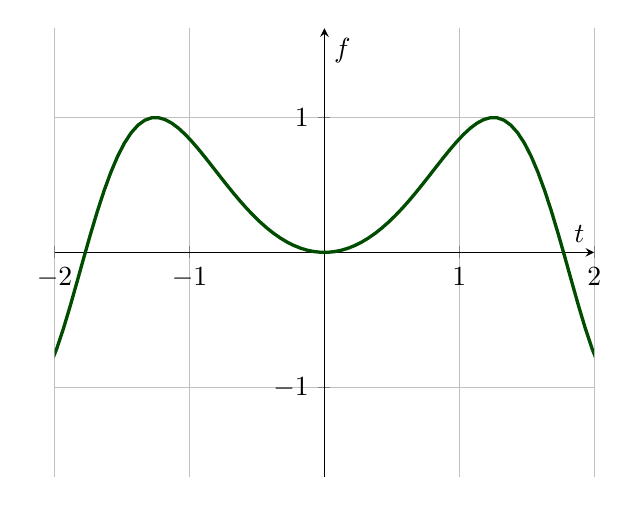
\begin{tikzpicture}
	\begin{axis}[axis lines=middle, axis equal, grid=both, xmin = -2, xmax = 2, ymin = -1, ymax = 1, xlabel = $t$, ylabel = $\operatorname{f}$]
		\addplot[black!70!green, very thick, samples = 200] {sin(deg(x^2))} node[above, red] at (10, 10) {$f$};
	\end{axis}
\end{tikzpicture}} & \scalebox{0.45}{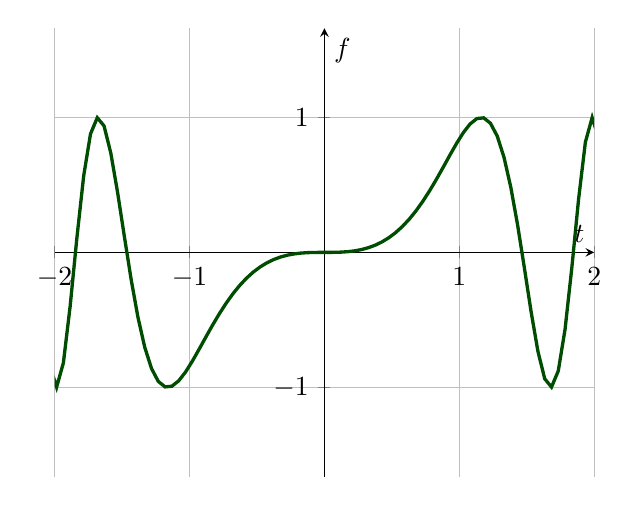
\begin{tikzpicture}
	\begin{axis}[axis lines=middle, axis equal, grid=both, xmin = -2, xmax = 2, ymin = -1, ymax = 1, xlabel = $t$, ylabel = $\operatorname{f}$]
		\addplot[black!70!green, very thick, samples = 200] {sin(deg(x^3))} node[above, red] at (100, 100) {$f$};
	\end{axis}
\end{tikzpicture}}\\[3pt]
					\hline
					achsensymmetrisch & punktsymmetrisch\\[3pt]
					$\displaystyle f(t) = f(-t)$ & $f(t) = -f(-t)$\\[3pt]
					\hline
					Beispiel: $\displaystyle \cos$ & Beispiel: $\sin$\\[3pt]
					\hline
					$\displaystyle \int\limits_{0}^{T} f(t) dt = 2 \cdot \int\limits_{0}^{T/2} f(t) dt$ & $\displaystyle \int\limits_{0}^{T} f(t) dt = 0$\\[3pt]
					\hline
				\end{tabular}
			\end{minipage}
			\begin{minipage}[]{0.5\textwidth}
				\textbf{Rechnen mit geraden und ungeraden Funktionen:}\\[3pt]
				\begin{tabular}{|lclcl|}
					\hline
					gerade & $\cdot$ & gerade & $=$ & gerade\\[3pt]
					ungerade & $\cdot$ & ungerade & $=$ & gerade\\[3pt]
					gerade & $\cdot$ & ungerade & $=$ & ungerade\\[3pt]
					\hline
				\end{tabular}\\[3pt]
				\textbf{Fourierkoeffizienten $a_n$, $b_n$:}\\[3pt]
				\begin{tabular}{|l|ll|}
					\hline
					$f(t)$		&  $a_n$, $b_n$ & \\[3pt]
					\hline
					gerade		& $b_n = 0$ ; & $\displaystyle a_n = \dfrac{4}{T} \int\limits_{0}^{T/2} f(t) \cdot \cos(n \omega_f t) dt$\\[3pt]
					\hline
					ungerade	& $a_n = 0$ ; & $\displaystyle b_n = \dfrac{4}{T} \int\limits_{0}^{T/2} f(t) \cdot \sin(n \omega_f t) dt$\\[3pt]
					\hline
				\end{tabular}
			\end{minipage}
		\subsubsection{Linearität}
			$f(t)$, $g(t)$ und $h(t)$ sind $T$-periodische Funktionen.\\[3pt]
			\begin{tabular}{lllll}
				Wenn gilt: 
				&
				\fbox{$h(t) = r \cdot f(t) + s \cdot g(t)$} 
				&
				$\Rightarrow$ 
				&
				\begin{tabular}{l}
					\fbox{$a_n^{(h)} = r \cdot a_n^{(f)} + s \cdot a_n^{(g)}$}\\[3pt]
					\fbox{$b_n^{(h)} = r \cdot b_n^{(f)} + s \cdot b_n^{(g)}$}\\[3pt]
				\end{tabular}
				&
				$r$, $s \in \mathbb{R}$
			\end{tabular}
		\subsubsection{Streckung / Stauchung}
			$f(t)$ ist eine $T$-periodische Funktion und $g(t)$ eine $\dfrac{T}{r}$-periodische Funktion.\\[3pt]
			\begin{tabular}{llllllll}
				$\Rightarrow$ 
				&
				\fbox{$g(t) = f(r \cdot t)$} 
				&
				$\Rightarrow$ 
				&
				\begin{tabular}{l}
					\fbox{$a_n^{(g)} = a_n^{(f)}$}\\[3pt]
					\fbox{$b_n^{(g)} = b_n^{(f)}$}\\[3pt]
				\end{tabular} 
				&
				$0 < r \in \mathbb{R}$
				&
				$\Rightarrow \left\lbrace 
					\begin{array}{l}
						r < 1 \rightarrow \text{Streckung}\\[3pt]
						r > 1 \rightarrow \text{Streckung}\\[3pt]
					\end{array}\right.$
				&
				und
				&
				\fbox{$\omega_g = \dfrac{2 \pi r}{T} = \omega_f \cdot r$}
			\end{tabular}
		\subsubsection{Verschiebung}
			$g(t)$ ist eine von $f(t)$ um $t_0$ verschobene T-periodische Funktion 
			$\Rightarrow \left\lbrace 
				\begin{array}{l}
					f(t + t_0) \rightarrow \text{Verschiebung nach links}\\[3pt]
					f(t - t_0) \rightarrow \text{Verschiebung nach rechts}\\[3pt]
				\end{array} 
			\right.$\\[3pt]
			\begin{tabular}{llllll}
				$\Rightarrow$
				&
				\fbox{$g(t) = f(t + t_0)$}
				&$\Rightarrow$
				&\begin{tabular}{l}
					\fbox{$a_n^{(g)} = \cos(n \omega_f t_0) \cdot a_n^{(f)} + \sin(n \omega_f t_0) \cdot b_n^{(f)}$}\\[6pt]
					\fbox{$b_n^{(g)} = -\sin(n \omega_f t_0) \cdot a_n^{(f)} + \cos(n \omega_f t_0) \cdot b_n^{(f)}$}\\[3pt]
				\end{tabular}
				&
				;
				&
				\fbox{$b_0 = 0$}\\[3pt]
			\end{tabular}
		
		\subsection{Konvergenz der Fourierreihen}
			\subsubsection{Optimalität der Fourierreihe (Approximation)}
				\begin{minipage}[b]{0.55\textwidth}
					\textbf{Abstand zwischen zwei Funktionen $f$ und $g$:}\\[3pt]
					\fbox{$\displaystyle||f - g|| = \sqrt{\dfrac{2}{T} \int\limits_{0}^{T} \left[ f(t) - g(t) \right]^2 dt}$}\\[3pt]
					Abstand $||f - g||$ zweier Funktionen kann klein sein, obschon sich die Funktionswerte stellenweise stark unterscheiden!
				\end{minipage}
				\begin{minipage}[]{0.45\textwidth}
					\scalebox{0.8}{\begin{tikzpicture}
	\begin{axis}[axis lines=middle, axis equal, grid=both, xmin=0, xmax=1, ymin=-2.5, ymax=1, xlabel = $t$, ylabel = $\operatorname{A}$]
		\addplot[name path=f, purple, very thick, samples=200] {sin(deg(x^2))} node[above, purple] at (180, 300) {$f$};
		\addplot[name path=g, cyan, very thick, samples=200] {sin(deg(2*x))*x} node[above, cyan] at (130, 280) {$g$};
		\addplot[orange!50] fill between[of=f and g];
	\end{axis}
\end{tikzpicture}}\\[3pt]
				\end{minipage}
				\textbf{Qualität der Approximation mit endlicher Fourierreihe:}\\[3pt]
				Die abbrechende Fourierreihe $s_m(t)$ approximiert $f$ hinsichtlich des Abstandes am besten!\\[3pt]
				\begin{tabular}{|lll|}
					\hline
					$\Rightarrow \quad \displaystyle ||s_m(t) - f(t)|| = ||\dfrac{a_0}{2} + \sum\limits_{n=1}^{m} [a_n \cdot \cos(n \omega_f t) + b_n \cdot \sin(n \omega_f t)] - f(t)||$ & $\rightarrow$ & wird minimal!\\[3pt]
					\textbf{Es gilt sogar:} & &\\[3pt]
					$\displaystyle \lim_{n \to \infty} ||\dfrac{a_0}{2} + \sum\limits_{n=1}^{m} [a_n \cdot \cos(n \omega_f t) + b_n \cdot \sin(n \omega_f t)] - f(t)|| = 0$ & &\\[3pt]
					\hline
				\end{tabular}\\[3pt]
				\begin{minipage}[t]{0.5\textwidth}
					\textbf{Parseval’sche Gleichung:}\\[3pt]
					\fbox{$\displaystyle \dfrac{a_0^2}{2} + \sum\limits_{n=1}^{m} (a_n^2 + b_n^2) = \dfrac{2}{T} \cdot \int\limits_{0}^{T} [f(t)]^2 dt = ||f||^2$}
				\end{minipage}
				\begin{minipage}[t]{0.5\textwidth}
					\textbf{Gliedweises Differenzieren und Integrieren:}
					\begin{framed}
						Funktion $f$ ist 2-mal stetig differenzierbar\\[3pt]
						$\Rightarrow$ man darf Fourierreihe von $f$:
						\begin{itemize}
							\item[$-$] \textbf{gliedweises integrieren}
							\item[$-$] \textbf{$(k-2)$-mal gliedweise differenzieren}
				 		\end{itemize}
					\end{framed}
				\end{minipage}
				\textbf{Nullfolgen $a_n$ und $b_n$:}\\[3pt]
				Die Fourierkoeffizienten $a_n$ und $b_n$ bilden eine Nullfolge:\\[3pt]
				\fbox{$\displaystyle \lim_{n \to \infty} a_n = \lim_{n \to \infty} \dfrac{2}{T} \cdot \int\limits_{0}^{T} f(t) \cdot \cos(n \omega_f t) dt = 0$}
				\fbox{$\displaystyle \lim_{n \to \infty} b_n = \lim_{n \to \infty} \dfrac{2}{T} \cdot \int\limits_{0}^{T} f(t) \cdot \sin(n \omega_f t) dt = 0$}\\[3pt]
				$\Rightarrow$ Je häufiger $f$ stetig differenzierbar ist, desto schneller gehen $a_n$ bzw. $b_n$ gegen $0$!\\[3pt]
				\begin{minipage}[t]{0.5\textwidth}
					\fbox{$|a_n| \leq \dfrac{c}{n^{k + 1}}$}
					\fbox{$|b_n| \leq \dfrac{c}{n^{k + 1}}$}
					$\begin{array}{l}
						c \in \mathbb{R}\\
						n \in \mathbb{N}\\
					\end{array}$
				\end{minipage}
				\begin{minipage}[t]{0.5\textwidth}
					\begin{tabular}{l}
						$(k - 1)$-mal stetig differenzierbar\\
						$k$-te Ableitung stückweise mit Limes stetig, monoton\\
					\end{tabular}
				\end{minipage}
			
			\subsubsection{Punktweise Kovergenz von Fourierreihen (Satz von Dirichlet)}
				\begin{minipage}[b]{0.65\textwidth}
					\begin{itemize}
						\item[$-$] Funktion $f(t)$ ist $T$-periodisch und stückweise stetig mit Limes.
						\item[$-$] Rechts- und linksseitige Ableitungen $\displaystyle \lim_{t \downarrow t_0} f'(t)$, $\displaystyle \lim_{t \uparrow t_0} f'(t)$ existierten.
					\end{itemize}
					$\Rightarrow$ \fbox{$\displaystyle FR[f(t_0)] \xrightarrow[]{n \to \infty} \dfrac{\displaystyle\lim_{t \downarrow t_0} f(t) + \displaystyle\lim_{t \uparrow t_0} f(t)}{2}$}
				\end{minipage}
				\begin{minipage}[]{0.35\textwidth}
					\scalebox{0.8}{\pgfplotsset{soldot/.style={color=blue,only marks,mark=*}} \pgfplotsset{holdot/.style={color=blue,fill=white,only marks,mark=*}}
\begin{tikzpicture}
	\begin{axis}[axis lines=middle, axis equal, grid=both, xlabel = $t$, ylabel = $\operatorname{f}$]
		\addplot[domain=0:4, blue] {sin(deg(x)) + 17};
		\addplot[domain=4:6, blue] {x};
		\addplot[domain=6:10, blue] {(x - 6)^2 - 5};
		\draw[dotted] (axis cs:4,16) -- (axis cs:4,4);
		\draw[dotted] (axis cs:6,6) -- (axis cs:6,-5);
		\addplot[holdot] coordinates{(0,0)(4,4)(6,-5)};
		\addplot[soldot] coordinates{(4,16)(6,6)(10,11)};
	\end{axis}
\end{tikzpicture}}\\[3pt]
				\end{minipage}
			
			\subsubsection{Gibbs-Phänomen}
				\begin{minipage}[b]{0.65\textwidth}
					\textbf{Gibbs'sches Phänomen:}\\[3pt]
					''Über- und Unterschiessen'' vor und nach einer Sprungstelle.\\[3pt]
					\textbf{Höhe der grössten überschwingenden Welle:}\\[3pt]
					Etwa $9\% (8.94\%)$ der gesamten Sprunghöhe.\\[3pt]
					\textbf{Anzahl Summanden $m \rightarrow \infty$:}\\[3pt]
					Grösste überschwingende Welle $\approx 9\%$, \textbf{klingt aber schneller aus.}
				\end{minipage}
				\begin{minipage}[]{0.35\textwidth}
					\scalebox{0.8}{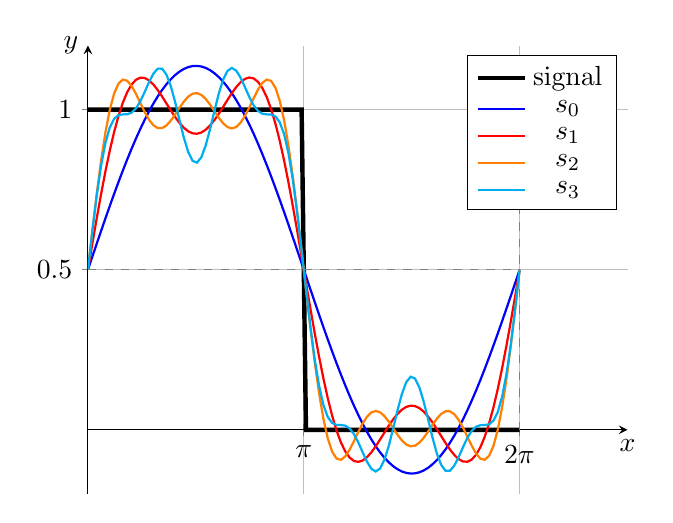
\begin{tikzpicture}
	\begin{axis}[
		xmin = 0, xmax = 2.5 * pi,
		ymin = -0.2, ymax = 1.2,
		domain = 0 : 2 * pi,
		grid=both,
		xlabel = $x$,
		ylabel = $y$,
		axis x line = center, 
		axis y line = center,
		every axis x label/.append style = {below},
		every axis y label/.append style = {left},
		samples = 100,
		xtick = {0, 3.14, 6.28},
		xticklabels = {$0$, $\pi$, $2\pi$},
		declare function = {
		  s(\x) = ifthenelse(\x < pi, 1, 0);
		  s0(\x) = 0.5 + (2 / pi) * sin(deg(\x);
		  s1(\x) = s0(\x) + (2 / pi) * sin(3 * deg(\x)) / 3.0));
		  s2(\x) = s1(\x) + (2 / pi) * sin(5 * deg(\x)) / 5.0));
		  s3(\x) = s1(\x) + (2 / pi) * sin(7 * deg(\x)) / 7.0));
		}, ]
		
		\addplot[ultra thick, black] {s(x)};
		\addplot[thick, blue] {s0(x)};
		\addplot[thick, red] {s1(x)};
		\addplot[thick, orange] {s2(x)};
		\addplot[thick, cyan] {s3(x)};
		\legend{signal, $s_0$, $s_1$, $s_2$, $s_3$};    
		
		% labels
		\draw[gray, dashed] (0, 0.5) -- (2 * pi, 0.5);
		\draw[gray, dashed] (2 * pi, 0) -- (2 * pi, 1);
	\end{axis}
\end{tikzpicture}}\\[3pt]
				\end{minipage}
		
		\subsection{Komplexe Darstellung der Fourierreihen (in $\mathbb{C}$)}
			\begin{minipage}[t]{0.5\textwidth}
				\textbf{Komplexe Fourierreihe:}\\[3pt]
				\fbox{$\displaystyle \sum\limits_{k=-\infty}^{\infty} c_k \cdot \mathrm{e}^{\mathrm{j} k \omega_f t}$}\\[3pt]
				\textbf{Umrechungsformeln ($a_n$, $b_n \rightarrow c_n$):}\\[3pt]
				\fbox{$c_n = \dfrac{a_n - \mathrm{j} b_n}{2}$} für $n = 0, 1, 2, 3, \cdots (b_0 = 0)$\\[3pt]
				\fbox{$c_{-n} = \overline{c_n} = \dfrac{a_n + \mathrm{j} b_n}{2}$} für $n = 1, 2, 3, \cdots (b_0 = 0)$\\[3pt]
			\end{minipage}
			\begin{minipage}[t]{0.5\textwidth}
				\textbf{Komplexe Fourierkoeffizienten:}\\[3pt]
				\fbox{$\displaystyle c_n = \overline{c_{-n}} = \dfrac{1}{T} \cdot \int\limits_{0}^{T} f(t) \cdot \mathrm{e}^{(\mathrm{j} n \omega_f t)} dt$} für $n = 0, 1, 2, 3, \cdots$\\[3pt]
				\textbf{Umrechnungsformeln ($c_n \rightarrow a_n$, $b_n$):}\\[3pt]
				\fbox{$a_n = 2 \operatorname{Re}(c_n) = c_n + c_{-n}$} für $n = 0, 1, 2, 3, \cdots$\\[3pt]
				\fbox{$b_n = -2 \operatorname{Im}(c_n) = \mathrm{j}(c_n + c_{-n})$} für $n = 1, 2, 3, \cdots$\\[3pt]
			\end{minipage}
		
			\subsubsection{Sätze zur Berechnung komplexer Fourierkoeffizienten}
				\begin{minipage}[t]{0.5\textwidth}
					\textbf{Symmetrie:}\\[3pt]
					\begin{tabular}{|l|l|l|}
						\hline
						$f(t)$ & $c_k$ & $arg(c_k)$\\[3pt]
						\hline
						gerade & $\displaystyle \operatorname{Im}[c_k] = 0 ;$ & $\displaystyle arg(c_k) = 0 \text{ oder } \pi$\\[3pt]
						\hline
						ungerade & $\displaystyle \operatorname{Re}[c_k] = 0 ;$ & $\displaystyle arg(c_k) = \pm \dfrac{\pi}{2}$\\[3pt]
						\hline
					\end{tabular}\\[6pt]
				\end{minipage}
				\begin{minipage}[t]{0.5\textwidth}
					\textbf{Linearität:}\\[3pt]
					Wenn gilt: \fbox{$h(t) = r \cdot f(t) + s \cdot g(t)$}\\[3pt]
					$\Rightarrow$ \fbox{$c_k^{(k)} = r \cdot c_k^{(f)} + s \cdot c_k^{(g)}$} $r$, $s \in \mathbb{R}$\\[6pt]
				\end{minipage}
				\begin{minipage}[t]{0.5\textwidth}
					\textbf{Streckung / Stauchung:}\\[3pt]
					Wenn gilt: \fbox{$g(t) = f(r \cdot t)$} $0 < r \in \mathbb{R}$\\[3pt]
					$\Rightarrow$ \fbox{$c_k^{(g)} = c_k^{(f)}$} und \fbox{$\omega_g = \dfrac{2 \pi r}{T} = \omega_f \cdot r$}
				\end{minipage}
				\begin{minipage}[t]{0.5\textwidth}
					\textbf{Verschiebung:}\\[3pt]
					Wenn gilt: \fbox{$g(t) = f(t + t_0)$}\\[3pt]
					$\Rightarrow$ \fbox{$c_k^{(g)} = \mathrm{e}^{\mathrm{j} k \omega_f t_0} \cdot c_k^{(f)}$} $k \in \mathbb{Z}$
				\end{minipage}
			
			\subsubsection{Optimalität komplexer Fourierreihe (Approximation)}
				\begin{minipage}[t]{0.5\textwidth}
					\textbf{Parseval'sche Gleichung:}\\[3pt]
					\fbox{$\displaystyle \sum\limits_{k=-\infty}^{\infty} |c_k|^2 = \dfrac{1}{T} \cdot \int\limits_{0}^{T} [f(t)]^2 dt$}\\[6pt]
				\end{minipage}
				\begin{minipage}[t]{0.5\textwidth}
					\textbf{Qualität der Approximation:}\\[3pt]
					\fbox{$\displaystyle \lim_{m \rightarrow \infty} \left|\left| \sum\limits_{k=-m}^{m} c_k \cdot \mathrm{e}^{\mathrm{j} k \omega_f t} - f(t) \right|\right| = 0$}\\[3pt]
				\end{minipage}
				\textbf{Nullfolge $c_k$, bzw. $c_n$:}\\[3pt]
				\begin{minipage}[t]{0.5\textwidth}
					\fbox{$\displaystyle \lim_{n \rightarrow \infty} c_n = \lim_{n \rightarrow \infty} \overline{c_{-n}} = \lim_{n \rightarrow \infty} \dfrac{1}{t} \cdot \int\limits_{0}^{T} f(t) \cdot \mathrm{e}^{(-\mathrm{j} n \omega_f t)} dt = 0$}\\[3pt]
				\end{minipage}
				\begin{minipage}[t]{0.5\textwidth}
					$\Rightarrow$ Je häufiger $f$ stetig differenzierbar ist,\\[3pt]
					desto schneller gehen $c_k$ bzw. $c_n$ gegen $0$!\\[3pt]
				\end{minipage}
				